\documentclass[letterpaper, 12pt]{article}
\usepackage[margin=1in]{geometry}
\usepackage{graphicx}
\usepackage{listings}
\graphicspath{{images/}{../Template/images/}}
\lstset{language=[Motorola68k]assembler,basicstyle=\ttfamily,frame=single}

\newcommand{\hwnumber}{Lab 3}
\newcommand{\duedate}{September 22nd, 2015}

\newcommand{\capper}{\begin{flushright}Aviles, Jean-Ralph \\ EEL3744 \\ Section 1539 \\ \duedate{} \\ \hwnumber{}\end{flushright}}

\begin{document}
\capper{}
\section*{Prelab Questions}
\begin{enumerate}
  \item What is the advantage of mirroring the input and output ports to
    \$8000 - \$9FFF (also known as partial address decoding)? What would be
    necessary if you wanted to only place the ports at 0x8000 and no place else? \\
    \hspace*{8pt} The advantage of using partial address decoding is that it makes
    our design less complicated. Instead of having to specify an exact address to
    decode we specify a range which makes our logic easier. If we wanted to place
    the ports at address 0x8000 and nowhere else it our decoding logic would need
    to use more then just CS0.
  \item Write the address decode equation to put the input and output ports at
    addresses 0x1000 - 0x7FFF.  \\
    \hspace*{8pt} I believe this is impossible because 0x1000 is at an address
    reserved for EEPROM and base addresses for Chip Selects must lie on a 4K
    boundary but ignoring that we would simply need to use the address lines
    that the CPLD has access to. Since 0x1000 starts with 0b0001 and 0x7FFF
    starts with 0b0111 we would need to add $\overline{A_{15}}$ to the logic
    selecting equation for the input and output ports in our schematics.
  \item What is the complete range of external memory on the XMEGA? \\
    \hspace*{8pt} According to the manual, the range of external memory
    addresses we have access to is from 0x3000 - 0xFFFFFF.
  \item The uPAD Proto Base is configured to use the EBI in SRAM ALE1 mode,
    which does not give us address bits A23:16. Which mode(s) can be used to
    access these higher address bits? Describe the change(s) necessary to use
    one of these modes. What additional hardware is needed, if any?
    \hspace*{8pt} If we set the EBI to SRAM ALE2 or ALE12 modes we would have
    access to those higher order bits. If we swapped over to the new mode we
    would need a new board to access all the new address bits we now have since
    we only have address to $A_{12} - A_{15}$.

\end{enumerate}
\section*{Problems Encountered}
It took me a bit to understand what was begin asked for the address decoding section. I think the lab was worded a bit weird. The decoding logic also was difficult to get right, also OSX El Capitan broke my Virtual Box.
\section*{Future Work/Applications}
We can now memory map any device we want to the board and multiplex them to conserve the number of pins we have on the board.
\section*{Appendix}
\subsection*{Input/Output Ports}
\begin{description}
\item [Start address] \hfill \\
\hspace*{8pt} 0x8000 so EBI\_CS0\_BASEADDR = 0x8000.
\item [End address] \hfill \\
\hspace*{8pt} 0x9FFF
\item [Address size] \hfill \\
  \hspace*{8pt} 0x9FFF - 0x8000 = 0x1FFF. 0x1FFF + 1 = 0x2000 = \textbf{8192}
  addresses. Since we are indexing 0x2000 addresses we'll need 13 address bits. \\
  EBI\_CS0\_CTRLA = 13.
\end{description}
\subsubsection*{CPLD Schematic}
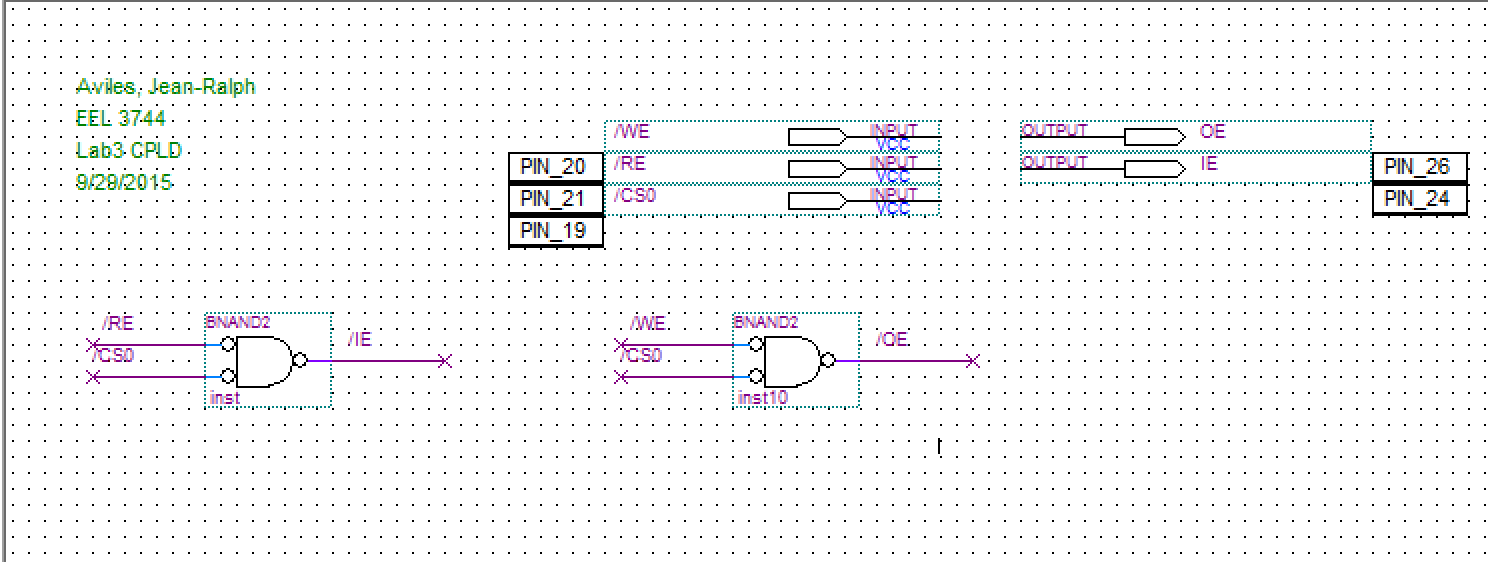
\includegraphics[width=1.0\textwidth,keepaspectratio=true]{CPLD}
\subsubsection*{Wiring diagram for input and output}
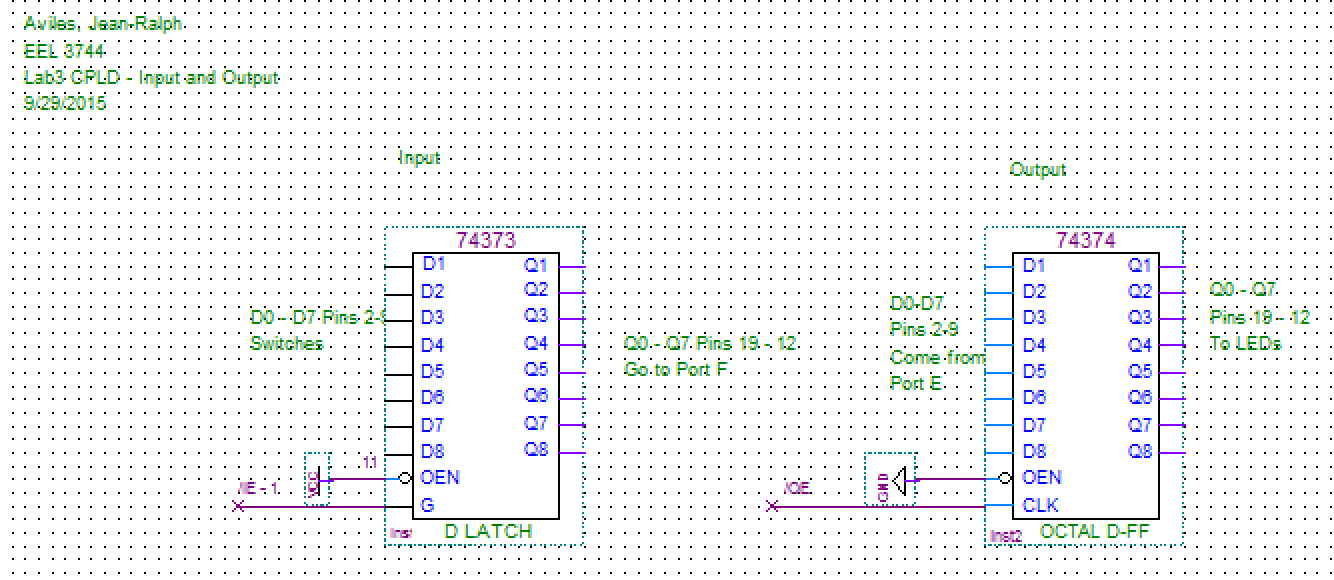
\includegraphics[width=1.0\textwidth,keepaspectratio=true]{IO}
\section*{Pseudocode/Flowcharts}
\subsection*{I/O Software}
\lstinputlisting{code/Lab3_JA.pc}
\section*{Programs}
\subsection*{I/O Software}
\lstinputlisting{code/Lab3_JA.asm}
\end{document}
